\section{Filter design}
In this section the process of designing digital filters is described. There will be distinguished between techniques for IIR and FIR filters. The section is concluded by a comparison of FIR and IIR filters. As described, ideal filters are not computable. Hence, the process of designing a filter is based on an approximation of the desired frequency response, which is based on computable polynomials and on a set of specifications for the filter. There exists different design methods to achieve this.

\subsection{IIR filters}
One common way of designing an IIR filter is to design the discrete-time filter from a corresponding continuous-time system. The method follows three main steps. 
\begin{itemize}
\item[1.] Specify the properties desired for the filter as filter specifications.
\item[2.] Hereby compute a ``prototype'' by a continuous-time system $H_c(j\Omega)$ that approximates the given properties. In this section it is done as a \textit{Butterworth filter}. Alternatives are the \textit{Chebyshev} and \textit{Elliptic} filters.
\item[3.] Transform the ``prototype'' into the discrete-time filter $H(\omega)$. In this section this is done with the \textit{Bilinear transformation}. An alternative is the \textit{impulse invariant method}.
\end{itemize}

The properties of a system are specified based on the desired application by considering what frequencies ideally are to pass the filter. Furthermore, it is important to specify how much the filter is allowed to vary from the ideal properties since an ideal filter is not a possibility. \\
Properties for an approximation to a lowpass filter is defined by a peak approximation error of the amplitude response of $\pm \ \delta_1$ of unity in a limited frequency band $0 \leq \Omega \leq \Omega_p $ and less than $\delta_2$ in the frequency band $\Omega_s \leq \Omega$ as illustrated in the tolerance scheme shown in figure \ref{fig:scheme}. Since the filter needs to be realizable, the transition band cannot be of zero width as it is for the ideal filter.
\frede{Trine ændrer positionen af "Stopband" i figuren}
\begin{figure}[H]
\centering
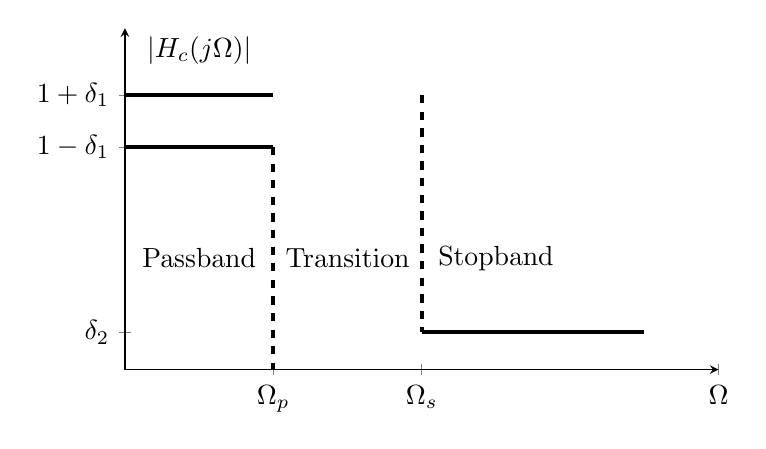
\begin{tikzpicture}[scale=1]
\begin{axis}[
scale=1.1,
unit vector ratio*=1 1 1,
axis lines = middle,
xtick={0,2,4,8},
xticklabels={$0$,$\Omega_p$,$\Omega_s$,$\Omega$},
ytick={0.5,3,3.7},
yticklabels={$\delta_2$,$1-\delta_1$,$1+\delta_1$},
xmin=0,
xmax=8,
ymin=0,
ymax=4.6]
\node at (axis cs:1,4.3) {$|H_c(j\Omega)|$};
\draw[line width=0.5mm](axis cs:0,3.7)--(axis cs:2,3.7);
\draw[line width=0.5mm](axis cs:0,3)--(axis cs:2,3);
\draw[line width=0.5mm, dashed](axis cs:2,3)--(axis cs:2,0);
\draw[line width=0.5mm, dashed](axis cs:4,3.7)--(axis cs:4,0.5);
\draw[line width=0.5mm](axis cs:4,0.5)--(axis cs:7,0.5);
\node at (axis cs:1,1.5) {Passband};
\node at (axis cs:3,1.5) {Transition};
\node at (axis cs:5.0,1.5) {Stopband};
\end{axis}
\end{tikzpicture}
\caption{Specifications for the amplitude response $|H_c(j\Omega)|$.}
\label{fig:scheme}
\end{figure}

The predefined Butterworth filter is a lowpass filter approximation used to fit the filter to the requirements. For the Butterworth filter the squared amplitude response is defined as follows:
\begin{align} \label{eq:butter}
|H_c(j\Omega)|^2=\frac{1}{1+\left( \frac{j\Omega}{j\Omega_c}\right)^{2N}}.
\end{align}

The filter is characterised by the following three properties:
\begin{align*}
1.& \ \ \ |H_c(j\Omega)|^2 \left|\begin{matrix}
\\
\Omega=0
\end{matrix}\right. = 1 \ \  \forall \ N. \\
2.& \ \ \ |H_c(j\Omega)|^2 \left|\begin{matrix}
\\ 
\Omega=\Omega_c
\end{matrix}\right. = \dfrac{1}{2} \ \ \forall \ N. \\
3.& \ \ \ \text{The amplitude response is monotonic in the pass- and stopbands.}
\end{align*}

As the order $N$ of the filter increases, the characteristics become sharper and the filter approximates the ideal lowpass filter. This is illustrated in figure \ref{fig:butter}. By \eqref{eq:butter} it is possible to compute the order necessary for the system to fulfil the specifications.            
\begin{figure}[H]
    \centering
    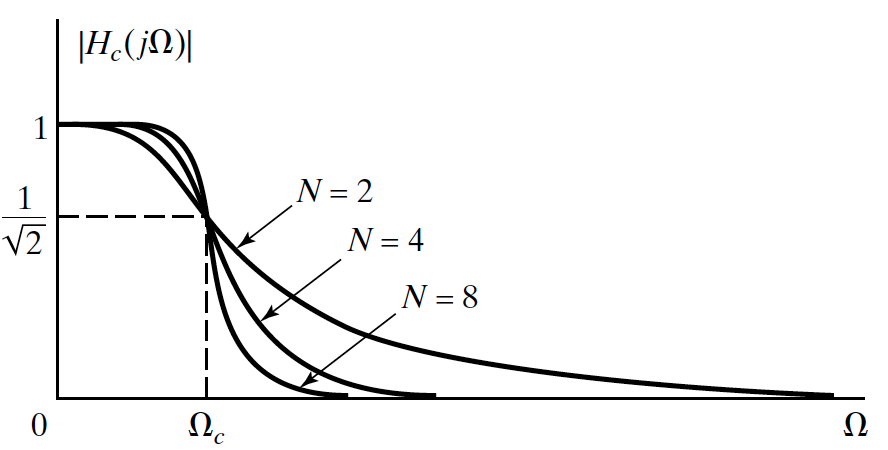
\includegraphics[width = 0.6\textwidth]{figures/butterworth.png}
    \caption{Amplitude response of Butterworth filter depending on the order $N$.}
    \label{fig:butter}
\end{figure}

An important remark is that $|H_c(j\Omega_c)| = \frac{1}{\sqrt{2}}$ corresponds to $20\cdot \log\left(\frac{1}{\sqrt{2}}\right) = -3$ dB. \\
\eqref{eq:butter} is transformed to the $s$-domain by substituting $s = j\Omega$:
\begin{align} \label{eq:Butter_trans}
|H_c(s)|^2 = \dfrac{1}{1+\left( \frac{s}{j\Omega_c}\right)^{2N}}.
\end{align}

By letting the denominator in \eqref{eq:Butter_trans} equal zero it is possible to determine the poles $s_k$ of the system:
\begin{align*}
1+\left( \dfrac{s}{j\Omega_c}\right)^{2N} &= 0 \ \  \Rightarrow  \ \ \frac{s}{j \Omega_c} = \sqrt[2N]{-1} \ \ \Rightarrow 
\end{align*}
\begin{align*}
s_k = (-1)^{\frac{1}{2N}} \left( j\Omega_c \right) = \Omega_c\text{e}^{ \left( \frac{j\pi}{2N} \right) \left( 2k+ N-1 \right) }, \ \ k=0,1,\ ... \ , 2N-1.
\end{align*}

The poles are placed equally along the circle of radius $\Omega_c$ in the $s$-plane. By only considering the poles in the left half plane, $H_c(s)$ can be constructed as a stable system:
\begin{align*}
H_c(s)=\dfrac{G}{\prod_{k=1}^{N}(s-s_k)},
\end{align*}

where $G$ is the gain constant determined as the 0 dB DC-gain, that is the value satisfying that $|H(0)| = 1$. After the continuous-time filter $H_c(s)$ been constructed, the next step is the transformation of the filter to the $z$-domain. The Bilinear transformation is a method that allows a direct transformation between the $s$- and $z$-domains. The principle of the transformation is that the entire imaginary axis $j\Omega$ of the $s$-plane is mapped onto the $z$-plane as the unit circle.
\\\\
The bilinear transformation is defined by 
\begin{align*}
s=\frac{2}{T_d}\left(\frac{1-z^{-1}}{1+z^{-1}}\right)
\end{align*}

such that 
\begin{align} \label{eq:bilinear}
H_c\left[\frac{2}{T_d}\left(\frac{1-z^{-1}}{1+z^{-1}}\right)\right]=H_c(z). 
\end{align}

Because $-\infty \leq \Omega \leq \infty $ is mapped to $-\pi \leq \omega \leq \pi$ the transformation is non-linear. This can also be seen from \eqref{eq:bilinear}, and the non-linearity necessarily involves some frequency distortion. Therefore, the use of this method is restricted to situations where this is acceptable or can be compensated. Compensation can be done by the concept of prewarping, which uses the relation
\begin{align*}
\Omega_{c_{new}} = \dfrac{2}{T_d} \tan \left( \dfrac{\omega_c}{2} \right),
\end{align*}
where $\omega_c$ is the discrete cut-off frequency. Hereby it is possible to determine a new $\Omega_c$ to the time-continuous filter, which ensures that the discrete $\omega_c$ fits the specifications. \\\\
An important property of the bilinear transformation is that stability is preserved if the time-continuous filter is stable.

\subsection{FIR filter} \label{subsec:FIR}
Design of FIR filters are in contrast to IIR filters based on approximating the desired time-discrete frequency response directly. By this method it is possible to guarantee a general linear phase of the system. The method uses the window method, which is described below.

\subsubsection{The window method}
The window method is considered a simple method for designing FIR filters. The method takes off from the ideal frequency response $H_d$, which is defined to be equal to one in passbands and zero in stopbands corresponding to the desired cut-off frequencies as in section \ref{sec:basic_filter}. Hereby the idealized impulse response $h_d[n]$ is obtained by the inverse Fourier transform of the desired frequency response:
\begin{align*}
h_d[n]=\frac{1}{2\pi}\int_{-\pi}^{\pi} H_d(\omega)\text{e}^{j\omega n} d\omega.
\end{align*}

$H_d(\omega)$ usually results in an impulse response of infinite length caused by the discontinuities at the boundaries between the pass- and stopbands. To compute a finite causal system as a FIR filter on behalf of the desired impulse response $h_d[n]$, the realisable impulse response $h[n]$ of the FIR filter is determined as a product of the impulse response $h_d[n]$ and a finite duration window $w[n]$ such that
\begin{align*}
h[n]=h_d[n]w[n], \ \ w[n] =
\begin{cases}
f[n], &\ 0 \leq n \leq M \\
0, &\ Otherwise
\end{cases}.
\end{align*}

Hereby the frequency response from \eqref{eq:type1} with the symmetry point at $\frac{M}{2}$ is truncated by the window, which introduces Gibbs phenomenon shown in figure \ref{fig:lowpass_real}. By this truncation the impulse response of a finite filter of order $M$ is determined such that
\begin{align*}
h[n]= 
\begin{cases}
h_d[n]w[n], &\ 0 \leq n \leq M \\
0, &\ Otherwise
\end{cases}.
\end{align*}

This is illustrated by an example of the simple \textit{rectangular window} defined as 
\begin{align*}
w[n] =
\begin{cases}
1, &\ 0 \leq n \leq M \\
0, &\ Otherwise
\end{cases}.
\end{align*}

By the Fourier transform this gives the following expression.
\begin{align*}
W\left(\omega\right) = \sum_{n=0}^{M} \text{e}^{-j\omega n} = \dfrac{1 - \text{e}^{-j\omega(M+1)}}{1 - \text{e}^{-j\omega}} = \text{e}^{-j\omega \frac{M}{2}} \frac{ \sin \left( \frac{\omega \left( M+1 \right)}{2} \right)}{\sin \left( \frac{\omega}{2} \right)}.
\end{align*}

Figure \ref{fig:rect_db} illustrates the so-called main and side lobes by a decibel plot of the amplitude response corresponding to the rectangular window.

\begin{figure}[H]
\centering
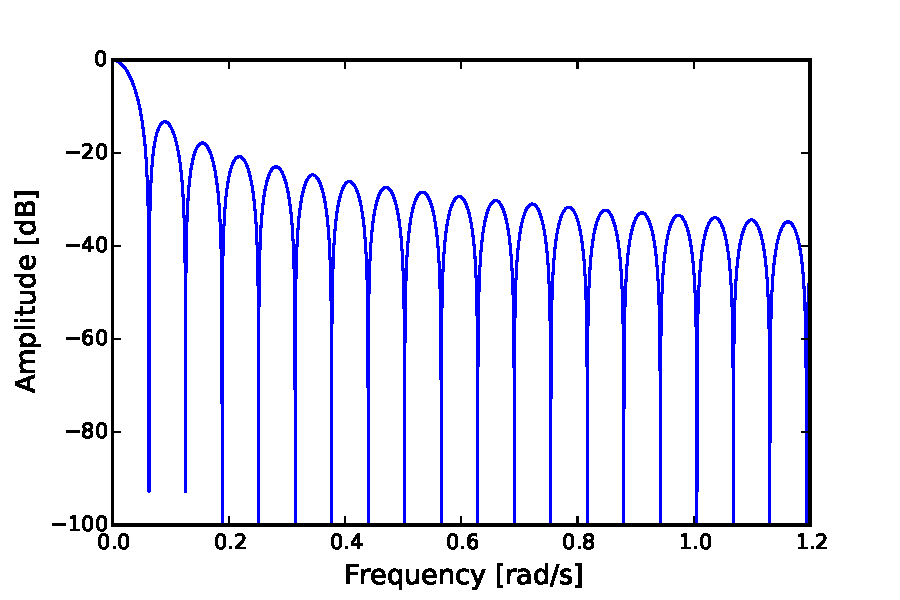
\includegraphics[width=0.7\textwidth]{figures/dbplots/rect.pdf}
\caption{Amplitude response in dB of the rectangular window of order $M=100$.}
\label{fig:rect_db}
\end{figure}

%
%\begin{figure}[H]
%\centering
%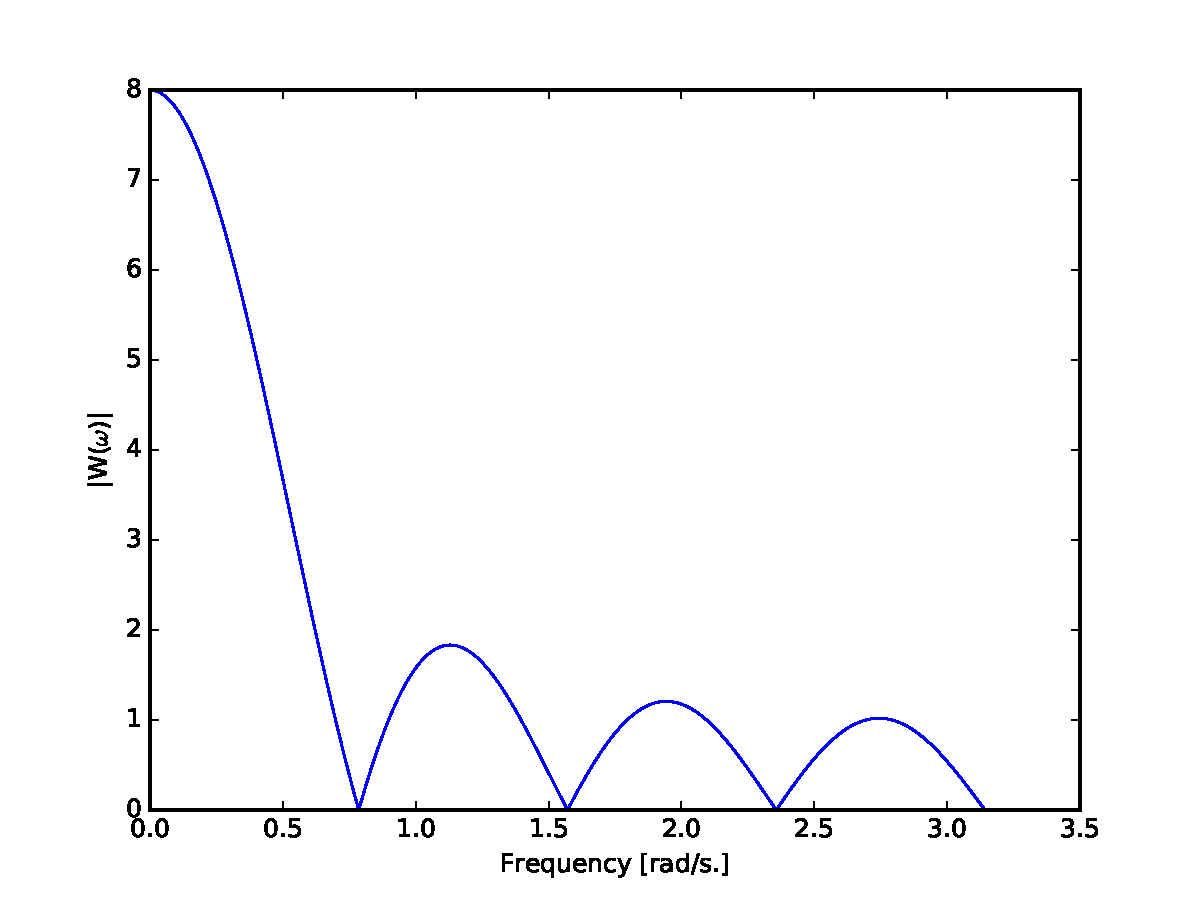
\includegraphics[scale=0.4]{figures/filter_teori/W_rect.pdf}
%\caption{Absolute amplitude response of the rectangular window of order $M=8$.}
%\label{fig:W_rect}
%\end{figure}
The aim is to approximate the ideal frequency response, which is best done by letting the main lobe of $W(\omega)$ be as narrow as possible and the side lobes as small as possible \cite{page 558, DTSP}. This corresponds to minimizing the width of the transitionband and the ripples in the pass- and stopbands, respectively, but it is not possible to achieve both simultaneously. \\
By increasing the filter order $M$, the width of the main lope is decreased but the peak amplitude of the side lopes also increases. This indicates a trade-off between the width of the main lope and the peak amplitude of the side lopes.
\\ \\
Figure \ref{fig:lowpass_real} shows the actual amplitude response $|H(\omega)|$ of a lowpass filter, which is the Fourier transform of the product of the rectangular window and the desired impulse response
\begin{align*}
h_d[n] =
\begin{cases}
\dfrac{\sin\left(\omega_c\left(n - \frac{M}{2}\right)\right)}{\pi\left(n-\frac{M}{2}\right)}, \quad &n \neq \frac{M}{2} \\
\dfrac{\omega_c}{\pi}, \quad &n = \frac{M}{2}
\end{cases}.
\end{align*}

Equivalently, the frequency response $H(\omega)$ equals the convolution of $W(\omega)$ and $H_d(\omega)$. 

\begin{figure}[H]
\centering
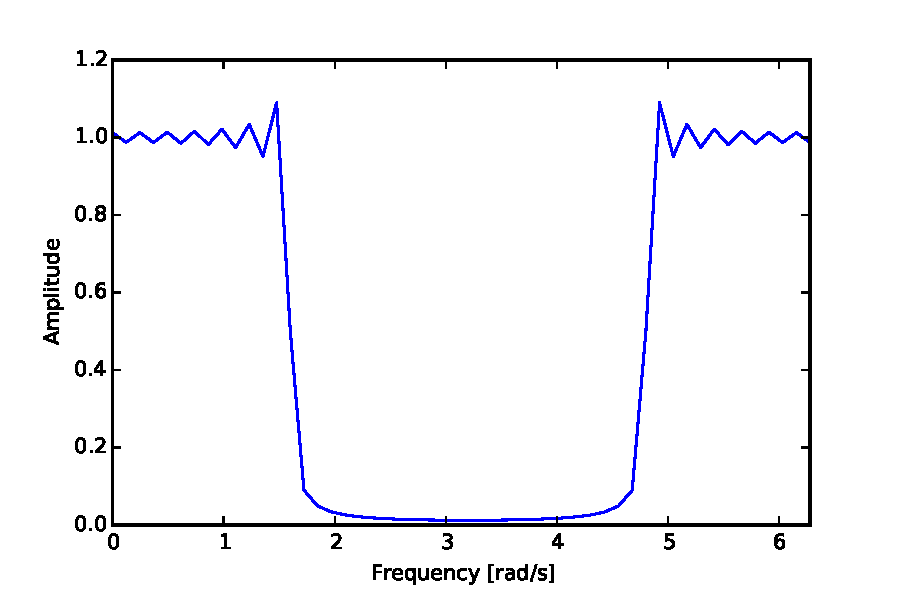
\includegraphics[width=0.7\textwidth]{figures/filter_teori/lowpass_real.pdf}
\caption{The amplitude response $|H(\omega)|$ of a FIR filter with the rectangular window, $M = 50$ and $\omega_c = \frac{\pi}{2}$. The Gibbs phenomenon is manifested through the ripples in the passband.}
\label{fig:lowpass_real}
\end{figure}

\subsubsection{Different types of windows}
The rectangular window is one out of many windows, all of which have different properties. The oscillations in $|H(\omega)|$ is a result of Gibbs phenomenon. Due to the convergence of the Fourier series this can be improved by convolving the desired frequency response with the Fourier transform of a less abrupt window. By narrowing each end of the window smoothly towards zero, the peak amplitude of the side lopes are remarkably decreased, although this will still result in the trade-off between the main lobe and the side lobes. \\
In table \ref{tab:window} in appendix \ref{appE} five commonly used windows are defined. Furthermore, the windows in time are shown in figure \ref{fig:win_type}, and the corresponding amplitude responses in dB of four of the windows are shown in figure \ref{fig:windows}.

\begin{figure}[H]
\centering
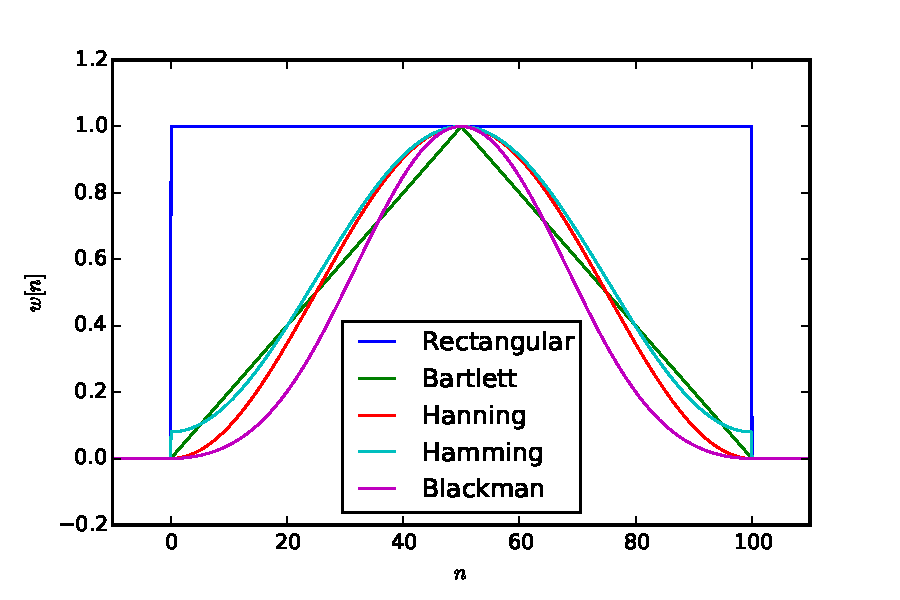
\includegraphics[width=0.7\textwidth]{figures/filter_teori/window_types.pdf}
\caption{Window functions in the time domain.}
\label{fig:win_type}
\end{figure}

\begin{figure}[H]
\centering
\begin{subfigure}{0.49\textwidth}
\centering
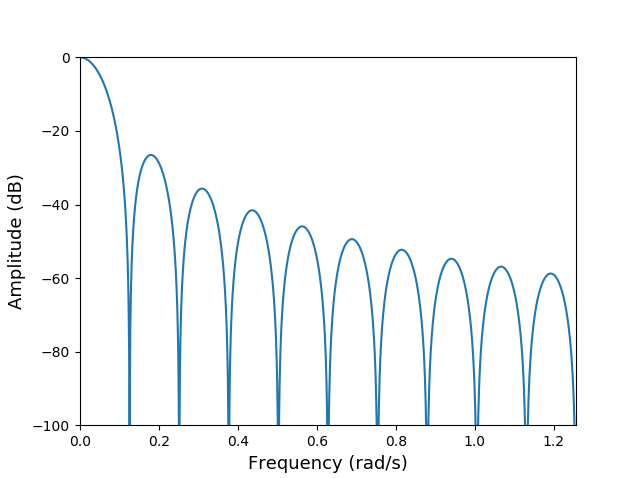
\includegraphics[width=\textwidth]{figures/dbplots/bartlett.png}
\caption{The Bartlett window.}
\label{fig:bartlett_db}
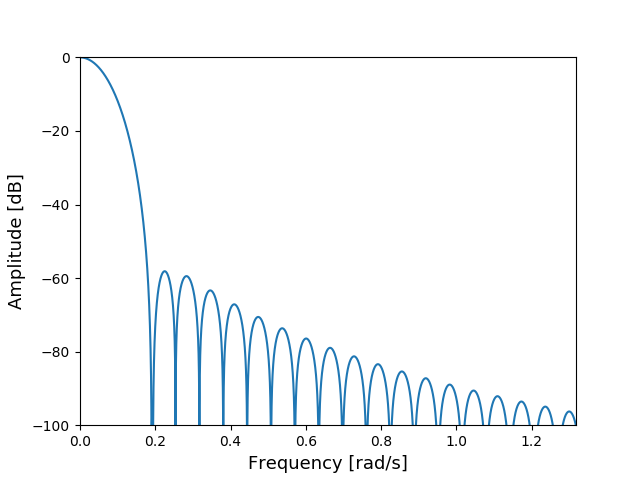
\includegraphics[width=\textwidth]{figures/dbplots/blackman.png}
\caption{The Blackman window.}
\label{fig:blackman_db}
\end{subfigure}
\begin{subfigure}{0.49\textwidth}
\centering
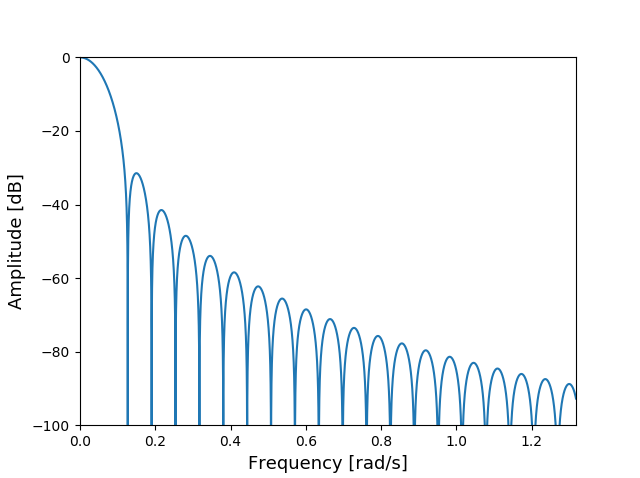
\includegraphics[width=\textwidth]{figures/dbplots/hann.png}
\caption{The Hann window.}
\label{fig:hann_db}
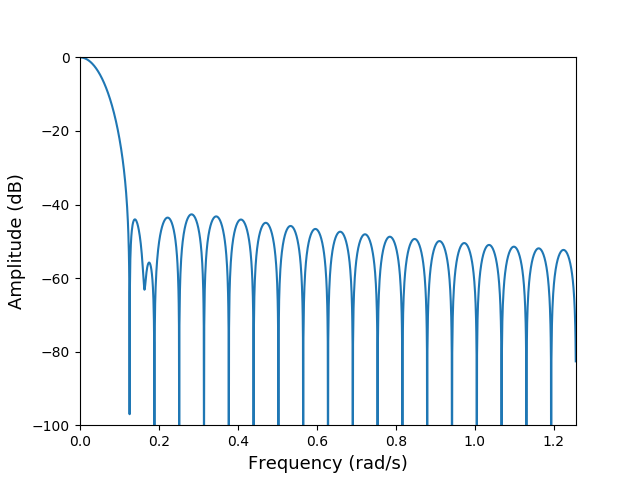
\includegraphics[width=\textwidth]{figures/dbplots/hamming.png}
\caption{The Hamming window.}
\label{fig:hamming_db}
\end{subfigure}
\caption{Plots of amplitude responses in dB of chosen windows of order $M=100$.}
\label{fig:windows}
\end{figure}

The defined windows all have the property of being symmetric around the point $\frac{M}{2}$. Hence, if the ideal impulse response is also symmetric the windowed impulse will be symmetric, which results in a frequency response with generalized linear phase. \\
To summarize, in this section it is seen that in order to design a FIR filter by the window method, the impulse response of the filter is obtained as the product of the desired impulse response and a window of a certain order, and one can vary the chosen window and the order of the filter until the desired specifications have been achieved.

\subsubsection{The Kaiser window method}
The Kaiser window design method considers the Kaiser window as the near-optimal window which -- compared to the other windows -- has two parameters; the length $M+1$ and a shape parameter $\beta$. This results in \textit{one} window where changing the parameters adjusts shape and length of the window. This is done in order to achieve the optimal trade-off between the peak amplitude of the side lopes and the width of the main lope \cite{page 566, DTSP}. The Kaiser window is defined as
\begin{align*}
w[n] =
\begin{cases}
\dfrac{I_0[\beta (1-[\frac{n-\alpha}{\alpha}]^2)^{\frac{1}{2}}]}{I_0(\beta)} , &\ 0 \leq n \leq M  \\ 
0, &\ \text{Otherwise}
\end{cases},
\end{align*}

where $\alpha=\frac{M}{2}$ and $I_0(\cdot)$ is the zero'th order modified Bessel function of the first kind \cite{page 566, DTSP}. Increasing $\beta$ tapers the window in the time domain, which results in smaller side lopes of the Fourier transform. Increasing $M$ causes the width of the main lope to increase without changing the peak amplitude of the side lopes. This is illustrated in figures \ref{fig:kaiser_beta} and \ref{fig:kaiser_order}, respectively.

\begin{figure}[H]
\centering
\begin{subfigure}{0.49\textwidth}
\centering
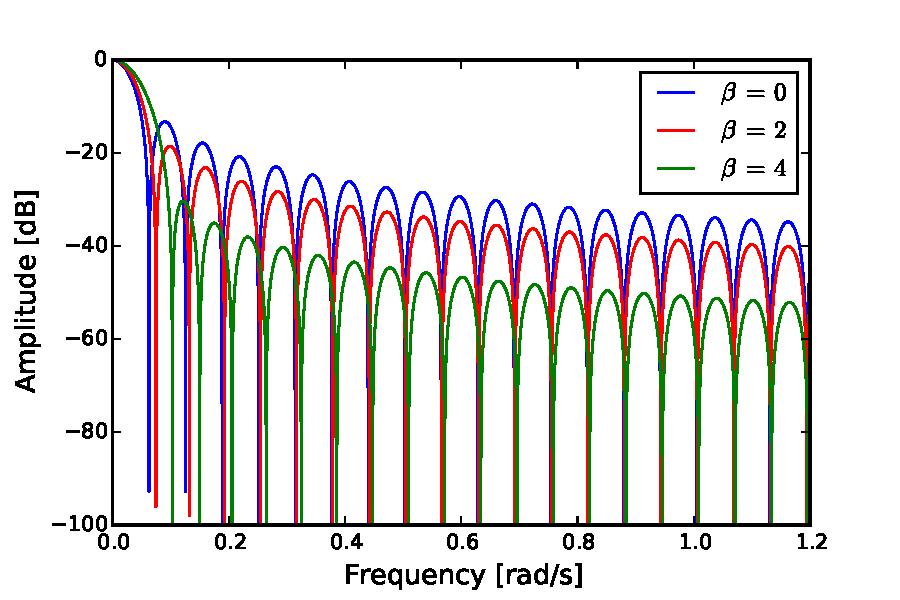
\includegraphics[width=\textwidth]{figures/dbplots/kaiser_beta.pdf}
\caption{}
\label{fig:kaiser_beta}
\end{subfigure}
\begin{subfigure}{0.49\textwidth}
\centering
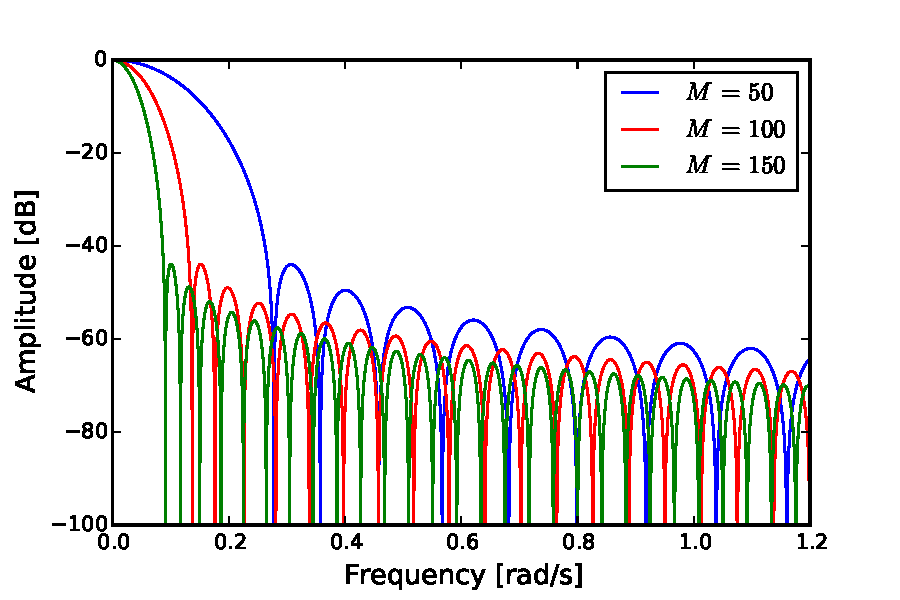
\includegraphics[width=\textwidth]{figures/dbplots/kaiser_order.pdf}
\caption{}
\label{fig:kaiser_order}
\end{subfigure}
\caption{\textbf{(a)} Amplitude responses of Kaiser windows in dB with $M=100$ and with $\beta=0$, $2$, and $4$. As $\beta$ increases the side lobes become smaller. \textbf{(b)} Amplitude responses of Kaiser windows in dB with $\beta=6$ and order $M=50$, $100$, and $150$. As $M$ increases the main lobe becomes narrower.}
\end{figure}
 
In order to determine values for $\beta$ and $M$ that satisfies the desired specifications of the filter, the following formulas are defined. Considering a lowpass filter with a fixed peak approximation error $\delta$ this gives a cut-off frequency $\omega_p$ of the passband defined as the highest frequency satisfying $|H(\omega)| \geq 1-\delta$ and a cut-off frequency $\omega_s$ of the stopband defined as the lowest frequency satisfying that $|H(\omega)| \leq \delta$. This gives a transitionband of width $\Delta \omega = \omega_s - \omega_p$. This is illustrated in figure \ref{fig:kaiser_spec}.
\\
Defining $A$ in [dB] by $\delta$ as $A = -20\log_{10} (\delta)$ it is possible to determine the value of $\beta$ on behalf of a specific value of $A$ as \cite{page 566, DTSP}
\begin{align*}
\beta =
\begin{cases}
0.1102\left( A-8.7 \right), &\ A \geq 50 \\
0.5843\left(A-21\right)^{0.4}+0.07886(A-21), &\ 21 \leq A \leq 50 \\
0.0, &\  A \leq 21 
\end{cases}
\end{align*}
       
Furthermore, $M$ must satisfy the relation
\begin{align}
M = \dfrac{A-8}{2.285\Delta \omega}.
\end{align}
Specifications for a lowpass filter are illustrated in figure \ref{fig:kaiser_spec}. Figure \ref{fig:kaiser_H} shows an example of the actual amplitude response computed by the use of the Kaiser window, which is designed to fulfil $\delta=0.01$, $\omega_p = 0.4\pi$, and $\omega_p = 0.5\pi$. This gives $M=46$ and $\beta \approx 3.4$. It is noted that there are fewer ripples compared to the rectangular window shown in figure \ref{fig:lowpass_real}.

\begin{figure}[H]
\centering
\begin{subfigure}{0.49\textwidth}
\centering
\begin{tikzpicture}[scale=1]
\begin{axis}[
scale=1.1,
unit vector ratio*=1 1 1,
axis lines = middle,
xtick={0,2,4,7,8},
xticklabels={$0$,$\omega_p$,$\omega_s$,$\pi$,$[rad/s]$},
ytick={0.5,3,3.7},
yticklabels={$\delta$,$1-\delta$,$1+\delta$},
xmin=0,
xmax=8,
ymin=0,
ymax=4.6]
\node at (axis cs:1,4.3) {$|H(\omega)|$};
\draw[line width=0.5mm](axis cs:0,3.7)--(axis cs:2,3.7);
\draw[line width=0.5mm](axis cs:0,3)--(axis cs:2,3);
\draw[line width=0.5mm, dashed](axis cs:2,3)--(axis cs:2,0);
\draw[line width=0.5mm, dashed](axis cs:4,3.7)--(axis cs:4,0.5);
\draw[line width=0.5mm](axis cs:4,0.5)--(axis cs:7,0.5);
\node at (axis cs:1,1.5) {};
\node at (axis cs:3,1.5) {};
\node at (axis cs:5.0,1.5) {};
\end{axis}
\end{tikzpicture}
\caption{}
\label{fig:kaiser_spec}
\end{subfigure}
\begin{subfigure}{0.49\textwidth}
\centering
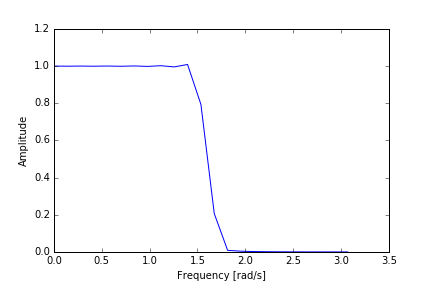
\includegraphics[width=\textwidth]{figures/filter_teori/kaiser_H.png}
\caption{}
\label{fig:kaiser_H}
\end{subfigure}
\caption{\textbf{(a)} illustration of specifications of a lowpass filter $H(\omega)$. \textbf{(b)} Amplitude response of $H(\omega)$ computed by a Kaiser window with $M=46$ and $\beta \approx 3.4$.}
\end{figure}

By this establishment of the Kaiser window method it is possible to design a FIR filter within a desired specification of $\delta$ with almost no iterations or trial and error. By adjusting the shape parameter $\beta$ it is possible to obtain a window equivalent to each of the windows defined in table \ref{tab:window} with a more narrow transition width, which could make the Kaiser window preferable \martin{Trine retter figuren med $\Delta \omega$}.

\section{Comparison of IIR and FIR filters}
This chapter concludes with a comparison of IIR and FIR filters by considering the advantages and disadvantages of the two types of filters.
\\ \\
The process of designing an IIR filter is rather complicated because the required order needs to be computed and the filter needs to be transformed as described. This design method leads to a recursive algorithm. By this method the amplitude response is the only parameter to be specified, and hence specific requirements for e.g. phase response or group delay are not guaranteed to be fulfilled by this kind of filter. However, once the filter has been designed, it is efficient and does not require a lot of computations.
\\ \\
The main advantages of a FIR filter is the guarantee of getting a precise generalized linear phase, which may be important in order to preserve the wave form of the original signal. The impulse response by the window method is straightforward to implement, although it is not pre-defined as a design equation, and iterations are thus often necessary before desired specifications are achieved.
\\ \\
When choosing the right filter design computational speed is often considered, which basically is related to the required order of the system and the amount of iterations with respect to the order.
\\ \\
By this it is clear that the choice of filter depends on the specific case and how different aspects are weighted. An IIR filter has advantages in efficiency and computations, which makes it preferable in cases, where the need of generalized linear phase is less significant, but in other cases linear phase and easy implementation of a FIR filter can be worth the extra computations.